%!TEX TS-program = xelatex

\documentclass[a4paper,12pt]{article}

%%% Работа с русским языком
\usepackage[english,russian]{babel}   %% загружает пакет многоязыковой вёрстки
\usepackage{fontspec}      %% подготавливает загрузку шрифтов Open Type, True Type и др.
\defaultfontfeatures{Ligatures={TeX},Renderer=Basic}  %% свойства шрифтов по умолчанию
\setmainfont[Ligatures={TeX,Historic}]{Calibri} %% задаёт основной шрифт документа
\setsansfont{Comic Sans MS}                    %% задаёт шрифт без засечек
\setmonofont{Courier New}
\usepackage{indentfirst}
\frenchspacing

\usepackage{ upgreek }
\renewcommand{\epsilon}{\ensuremath{\varepsilon}}
\renewcommand{\phi}{\ensuremath{\varphi}}
\renewcommand{\kappa}{\ensuremath{\varkappa}}
\renewcommand{\le}{\ensuremath{\leqslant}}
\renewcommand{\leq}{\ensuremath{\leqslant}}
\renewcommand{\ge}{\ensuremath{\geqslant}}
\renewcommand{\geq}{\ensuremath{\geqslant}}
\renewcommand{\emptyset}{\varnothing}

%%% Дополнительная работа с математикой
\usepackage{amsmath,amsfonts,amssymb,amsthm,mathtools} % AMS
\usepackage{icomma} % "Умная" запятая: $0,2$ --- число, $0, 2$ --- перечисление

%% Номера формул
%\mathtoolsset{showonlyrefs=true} % Показывать номера только у тех формул, на которые есть \eqref{} в тексте.
%\usepackage{leqno} % Нумерация формул слева	

%% Перенос знаков в формулах (по Львовскому)
\newcommand*{\hm}[1]{#1\nobreak\discretionary{}
	{\hbox{$\mathsurround=0pt #1$}}{}}

%%% Работа с картинками
\usepackage{graphicx}  % Для вставки рисунков
\graphicspath{{images/}}  % папки с картинками
\setlength\fboxsep{3pt} % Отступ рамки \fbox{} от рисунка
\setlength\fboxrule{1pt} % Толщина линий рамки \fbox{}
\usepackage{wrapfig} % Обтекание рисунков текстом
\usepackage{subcaption}

%%% Работа с таблицами
\usepackage{array,tabularx,tabulary,booktabs} % Дополнительная работа с таблицами
\usepackage{longtable}  % Длинные таблицы
\usepackage{multirow} % Слияние строк в таблице
\usepackage{float}% http://ctan.org/pkg/float

%%% Программирование
\usepackage{etoolbox} % логические операторы


%%% Страница
\usepackage{extsizes} % Возможность сделать 14-й шрифт
\usepackage{geometry} % Простой способ задавать поля
\geometry{top=20mm}
\geometry{bottom=20mm}
\geometry{left=30mm}
\geometry{right=15mm}
%
%\usepackage{fancyhdr} % Колонтитулы
% 	\pagestyle{fancy}
%\renewcommand{\headrulewidth}{0pt}  % Толщина линейки, отчеркивающей верхний колонтитул
% 	\lfoot{Нижний левый}
% 	\rfoot{Нижний правый}
% 	\rhead{Верхний правый}
% 	\chead{Верхний в центре}
% 	\lhead{Верхний левый}
%	\cfoot{Нижний в центре} % По умолчанию здесь номер страницы

\usepackage{setspace} % Интерлиньяж
\onehalfspacing % Интерлиньяж 1.5
%\doublespacing % Интерлиньяж 2
%\singlespacing % Интерлиньяж 1

\usepackage{lastpage} % Узнать, сколько всего страниц в документе.

\usepackage{soul} % Модификаторы начертания

\usepackage{hyperref}
\usepackage[usenames,dvipsnames,svgnames,table,rgb]{xcolor}
\hypersetup{				% Гиперссылки
	unicode=true,           % русские буквы в раздела PDF
	pdftitle={Отчет по самостоятельной работе},   % Заголовок
	pdfauthor={Самоделкина М.В., Ремизова А.П.},      % Автор
	pdfsubject={Отчет по самостоятельной работе},      % Тема
	pdfcreator={Самоделкина М.В., Ремизова А.П.}, % Создатель
	pdfproducer={Самоделкина М.В., Ремизова А.П.}, % Производитель
	pdfkeywords={keyword1} {key2} {key3}, % Ключевые слова
	colorlinks=true,       	% false: ссылки в рамках; true: цветные ссылки
	linkcolor=blue,          % внутренние ссылки
	citecolor=black,        % на библиографию
	filecolor=magenta,      % на файлы
	urlcolor=blue           % на URL
}
\makeatletter 
\def\@biblabel#1{#1. } 
\makeatother
\usepackage{cite} % Работа с библиографией
%\usepackage[superscript]{cite} % Ссылки в верхних индексах
%\usepackage[nocompress]{cite} % 
\usepackage{csquotes} % Еще инструменты для ссылок

\usepackage{multicol} % Несколько колонок

\usepackage{tikz} % Работа с графикой
\usepackage{pgfplots}
\usepackage{pgfplotstable}

% ГОСТ заголовки
\usepackage[font=small]{caption}
%\captionsetup[table]{justification=centering, labelsep = newline} % Таблицы по правобу краю
%\captionsetup[figure]{justification=centering} % Картинки по центру
\usepackage{ dsfont }

\newcommand{\tablecaption}[1]{\addtocounter{table}{1}\small \begin{flushright}\tablename \ \thetable\end{flushright}%	
\begin{center}#1\end{center}}

\newcommand{\imref}[1]{рис.~\ref{#1}}

\usepackage{multirow}
\usepackage{spreadtab}
\newcolumntype{K}[1]{@{}>{\centering\arraybackslash}p{#1cm}@{}}


\usepackage{xparse}
\usepackage{fancyvrb}

\RecustomVerbatimCommand{\VerbatimInput}{VerbatimInput}
{
	fontsize=\footnotesize    
}

\newcolumntype{?}[1]{!{\vrule width #1}}

\usepackage{tocloft}
\renewcommand{\cftsecleader}{\cftdotfill{\cftdotsep}}

\usepackage{pdfpages}

\usepackage{longtable}

\usepackage{adjustbox}
\begin{document}
\begin{titlepage}
	\begin{center}
		ПРАВИТЕЛЬСТВО РОССИЙСКОЙ ФЕДЕРАЦИИ \\
 		ФЕДЕРАЛЬНОЕ  ГОСУДАРСТВЕННОЕ АВТОНОМНОЕ \\
		ОБРАЗОВАТЕЛЬНОЕ УЧРЕЖДЕНИЕ ВЫСШЕГО ОБРАЗОВАНИЯ\\
		«НАЦИОНАЛЬНЫЙ ИССЛЕДОВАТЕЛЬСКИЙ УНИВЕРСИТЕТ\\
		«ВЫСШАЯ ШКОЛА ЭКОНОМИКИ»
	\end{center}
	
	\begin{center}
		\textbf{Московский институт электроники и математики}
		
		\textbf{Им. А.Н.Тихонова НИУ ВШЭ}
		
		\vspace{2ex}
		
		\textbf{Направление 01.03.04. Прикладная математика \\
			Бакалаврская программа <<Прикладная математика>>}
	\end{center}
	\vspace{1ex}	
	
	\vspace{1ex}
	\begin{center}
		\textbf{Домашняя работа \\
			по дисциплине <<Математическая теория страхования>>\\
			вариант 7
	}
	\end{center}	

	\vspace{2ex}
	\vfill
	
	\vspace{2ex}
	
	\begin{flushright}
		\textbf{Бригада №7:}
		
		\vspace{2ex}
		
		Ремизова Анна Петровна, 4 курс, БПМ174
		
		Самоделкина Мария Владимировна, 4 курс, БПМ174

	\end{flushright}

	\vspace{5ex}
	\begin{center}
		Москва \the\year \, г.
	\end{center}
	
\end{titlepage}
\addtocounter{page}{1}
\tableofcontents
\pagebreak

\section{Постановка задачи}
Для однородной группы из $n = 1000$ клинетов, имеющих вероятность страхового случая $p = 0,05$ и экспоненциальное распределение страховых выплат со средним $5$ денежных единиц, определить значение уровня $k$ для 
\begin{enumerate}
	\item безусловной франшизы
	\item условной франшизы,
\end{enumerate}
которое обеспечивает надежность $\beta = 98,5\%$ при размере собственного капитала $S = 35$. Коэффициент нагрузки равен $\alpha = 11\%$.

\section{Решение}
Страховые выплаты $X_1^0$ имеют распределение $F_1^0(x) = P\{X_1 \le x | X_1 > 0\}$. Так как $EX_1^0 = 5 = \frac{1}{\lambda}$, то $\lambda = 0,2$. Тогда запишем, что $F_1^0(x) = 1 - \exp(-0,2 x)$.

Определим вероятность ненулевого ущерба (новую вероятность страхового случая):
\[\hat{p} = 1 - \hat{F_1}(0) = 1 - F_1(k) = p (1 - F_1^0(k)) = p \exp(-0,2 k).\]

Зададим $n\hat{p} = np\exp(-0,2k) = 50 \exp (-0,2 k)$. Тогда если $n\hat{p} < 10$, то суммарный риск страховщика приближается сложно-пуассоновской аппроксимацией. Иначе если $n\hat{p} \ge 10$, то распределение суммарного риска страховщика заменяется нормальным распределением.

Найдем, при каких $k$ можно применять сложно-пуассоновскую или нормальную аппроксимацию. Из уравнения $50 \exp (-0,2 k) = 10$ находим, что $k \approx 8,05$. Таким образом, когда $k \le 8,05$, то применяем нормальную аппроксимацию, а в случае, когда $k > 8,05$ - сложно-пуассоновскую.

\subsection{Безусловная франшиза}
Функция дележа имеет вид $I(x) = \max\{0, x - k\}$, где $k \ge 0$ - уровень безусловной франшизы. 

\subsubsection{Нормальная аппроксимация}
$\hat{X} = \sum_{i=1}^{n} \hat{X}_i$ - суммарный ущерб страховщика. Тогда \[P\{S + (1 + \alpha)\hat{M} \ge \hat{X}\} = \Upphi_{\hat{M}, \hat{\sigma}}(S + (1 + \alpha)\hat{M}) = \Upphi_{0, 1}\left(\cfrac{S + \alpha\hat{M}}{\hat{\sigma}}\right) \ge \beta,\]
где $\hat{M} = E\hat{X} = nE\hat{X}_1 = n\hat{p}E\hat{X}_1^0 = np\exp(-0,2k)E\hat{X}_1^0$. Учитывая, что величина $\hat{X}_1^0$ при безусловной франшизе также имеет экспоненциальное распределение с параметром $\lambda = 0,2$, запишем, что $\hat{M} = 250\exp(-0,2k)$.
 
Также запишем, что $\hat{\sigma} = \sqrt{n D\hat{X}_1}$, так как ущербы независимы.  Далее распишем $n D\hat{X}_1 = n\hat{p} (D\hat{X}_1^0 + (1-\hat{p})E^2\hat{X}_1^0) = \lambda^{-2}np\exp(-0,2k)(2 - p\exp(-0,2k)) = 1250 \exp(-0,2k)(2 - 0,05\exp(-0,2k))$. 

От выражения $\Upphi_{0, 1}\left(\cfrac{35 +0,11\hat{M}}{\hat{\sigma}}\right) \ge 0,985$ перейдем к записи $\cfrac{35 +0,11\hat{M}}{\hat{\sigma}} \ge x_{0,985}$, где $x_{0,985}$ - квантиль стандартного нормального распределения. Далее необходимо решить следующее неравенство относительно $k$ ($k \ge 0$):
\[\cfrac{35 + 0,11 \cdot 250 \exp(-0,2 k)}{\sqrt{1250 \exp(-0,2k)(2 - 0,05\exp(-0,2k))}} \ge 2,17.\]

Получаем, что $k \ge 10,35$. Но для нормальной аппроксимации $k \in [0; 8,05]$. Таким образом, можно сделать вывод, что нет таких $k$, при которых можно применять нормальную аппроксимацию и которые обеспечивают требуемую надежность.

\subsubsection{Сложно-пуассоновская аппроксимация}
Рассмотрим $k > 8,05$, тогда можно применять сложно-пуассоновскую аппроксимацию суммарного ущерба страховщика. 

Распределение $\hat{X}$ приближается формулой 
\[\hat{F}(x) \approx \sum_{j = 0}^{s} \hat{F}_1^{0 * j}(x) \frac{\hat{\lambda}^j}{j!}\exp (-\hat{\lambda}),\]
где $\hat{\lambda} = n\hat{p}$, а $\hat{F}_1^{0 * j}(x)$ - $j$-кратная свертка ($\hat{F}_1^{0 * j}(x) = P\{\hat{X}_1^0 + \dots \hat{X}_j^0 \le x\}$).

Как было отмечено ранее, $\hat{F}_1^0(x) = 1 - \exp(-0,2 x), x>0$. Известно, что сумма независимых экспоненциально распределенных случайных величин имеет распределение Эрланга, то есть
\[\hat{F}_1^{0 * j}(x) = 1 - \sum_{i = 0}^{j - 1} \cfrac{(0,2 x)^i}{i!} \exp(-0,2x).\]

Формула из Леммы 1 позволяет определить значение $s$ в формуле для сложно-пуассоновской аппроксимации, чтобы погрешность аппроксимации не превосходила заданную точность (для дальнейших расчетов примем точность, равную $0,01$). Тогда минимальное число членов $s$ для аппроксимации находим из неравенства:
\[\frac{\hat{\lambda}^{s + 1} \min\{1, (s + 1)\exp(-\hat{\lambda})\}}{(s + 1)!} \le 0,01.\]
Так, для каждого значения $k$ должно быть свое значение $s$, чтобы не превосходить заданную погрешность. В работе использовалось значение $s = 14$ для всех $k$. При таком $s$ для любого рассматриваемого $k$ выполнялось неравенство из Леммы 1. То есть использовалось максимальное значение $s$, необходимое, для обеспечения требуемой точности аппроксимации для различных $k$ (для некоторых $k$ значение $s$ для заданной точности могло быть меньше $14$).

С помощью прикладного ПО найдем минимальное значение $k$, при котором выполняется следующее неравенство:
\[\hat{F}(S + (1 + \alpha)\hat{M}) \ge 0,985,\]
где $\hat{F}(x) \approx \sum_{j = 0}^{s} \left(1 - \sum_{i = 0}^{j - 1} \cfrac{(0,2 x)^i}{i!} \exp(-0,2x)\right) \cfrac{\hat{\lambda}^j}{j!}\exp (-\hat{\lambda})$.

Таким образом, с помощью программы на языке Python был получен уровень безусловной франшизы $k=13,36$. На графике (рис. \ref{fig:graph1}) представлена зависимость аппроксимации надежности страховщика $\hat{F}(x)$ от уровня безусловной франшизы $k$ при $s = 14$.

\begin{figure}[H]
	\centering
	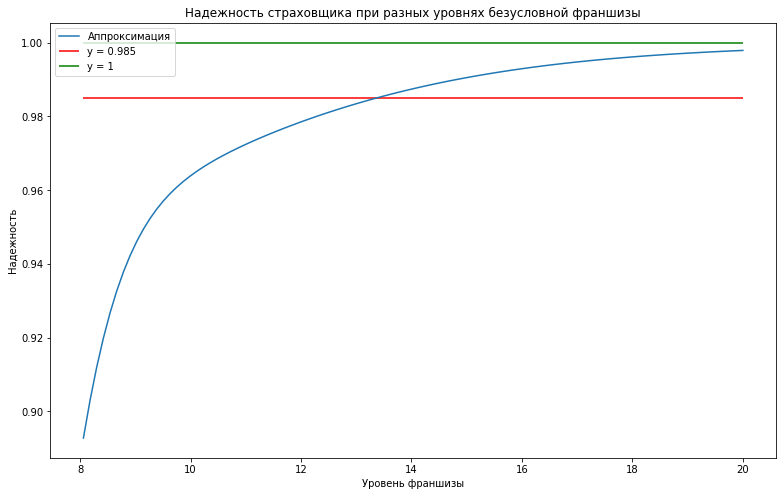
\includegraphics[width=0.9\linewidth]{graph1}
	\caption{Надежность страховщика при разных уровнях безусловной франшизы}
	\label{fig:graph1}
\end{figure}

\subsection{Условная франшиза}

В этом случае функция дележа разрывна и имеет вид: 

$$I(x) = 
	\begin{cases}
		0, &x \le k\\
		x, &x > k
	\end{cases}$$

где параметр $k \ge 0$ - уровень условной франшизы. В случае экспоненциальной страховой выплаты $X_1^0 \sim 1-\exp(-0,2x)$, тогда распределение $\hat{X}_1^0$:

$$\hat{F}_1^0(x) = 
\begin{cases}
	0, &x \le k\\
	1-\exp(-0,2(x-k)), &x > k
\end{cases}$$

совпадает с распределением случайной величины $k + {X}_1^0$.

\subsubsection{Нормальная аппроксимация}
$\hat{X} = \sum_{i=1}^{n} \hat{X}_i$ - суммарный ущерб страховщика. Тогда \[P\{S + (1 + \alpha)\hat{M} \ge \hat{X}\} = \Upphi_{\hat{M}, \hat{\sigma}}(S + (1 + \alpha)\hat{M}) = \Upphi_{0, 1}\left(\cfrac{S + \alpha\hat{M}}{\hat{\sigma}}\right) \ge \beta,\]
где $\hat{M} = E\hat{X} = nE\hat{X}_1 = n\hat{p}E\hat{X}_1^0 = np\exp(-0,2k)E\hat{X}_1^0$. Учитывая, что величина $\hat{X}_1^0$ при условной франшизе совпадает с распределением случайной величины $k + {X}_1^0$, где ${X}_1^0$ распределено экспоненциально $\lambda = 0,2$, то $E\hat{X}_1^0=E(X_1^0+k)=k+\frac{1}{\lambda}=k+5$. Таким образом, $\hat{M} = 50\exp(-0,2k)(k+5)$.

Также запишем, что $\hat{\sigma} = \sqrt{n D\hat{X}_1}$, так как ущербы независимы.  Далее распишем $n D\hat{X}_1 = n\hat{p} (D\hat{X}_1^0 + (1-\hat{p})E^2\hat{X}_1^0) = np\exp(-0,2k)(25 + (1 - p\exp(-0,2k))(k+5)^2) = 50 \exp(-0,2k)(25 + (1 - 0,05\exp(-0,2k))(k+5)^2)$, так как $D\hat{X}_1^0 = D (X_1^0+k) = DX_1^0 = \frac{1}{\lambda^2}$. 

От выражения $\Upphi_{0, 1}\left(\cfrac{35 +0,11\hat{M}}{\hat{\sigma}}\right) \ge 0,985$ перейдем к записи $\cfrac{35 +0,11\hat{M}}{\hat{\sigma}} \ge x_{0,985}$, где $x_{0,985}$ - квантиль стандартного нормального распределения. Далее необходимо решить следующее неравенство относительно $k$ ($k \ge 0$):
\[\cfrac{35 + 0,11 \cdot 50\exp(-0,2k)(k+5)}{\sqrt{50 \exp(-0,2k)(25 + (1 - 0,05\exp(-0,2k))(k+5)^2)}} \ge 2,17.\]

% для WolframAlpha (35 + 0.11*50exp(-0.2k)(k+5))/(sqrt(50exp(-0.2k)(25 + (1 - 0.05exp(-0.2k))(k+5)^2)))>=2.17

Получаем, что $k \ge 25,93$. Но для нормальной аппроксимации $k \in [0; 8,05]$. Таким образом, можно сделать вывод, что нет таких $k$, при которых можно применять нормальную аппроксимацию и которые обеспечивают требуемую надежность.

%TODO Вывод вставить куда-нибудь
В результате вычислений было получено, что уровень $k$ для условной франшизы больше, чем для безусловной. Действительно, при условной франшизе у компании большая ответственность и уменьшение среднего риска страховщика при том же уровне $k$ для условной франшизы всегда будет меньше.

\subsubsection{Сложно-пуассоновская аппроксимация}
Рассмотрим $k > 8,05$, тогда можно применять сложно-пуассоновскую аппроксимацию суммарного ущерба страховщика. 

Распределение $\hat{X}$ приближается формулой 
\[\hat{F}(x) \approx \sum_{j = 0}^{s} \hat{F}_1^{0 * j}(x) \frac{\hat{\lambda}^j}{j!}\exp (-\hat{\lambda}),\]
где $\hat{\lambda} = n\hat{p}$, а $\hat{F}_1^{0 * j}(x)$ - $j$-кратная свертка ($\hat{F}_1^{0 * j}(x) = P\{\hat{X}_1^0 + \dots + \hat{X}_j^0 \le x\}$).

Как было отмечено ранее, $\hat{F}_1^0(x) = 1-\exp(-0,2(x-k)), x>k$. Тогда: $\hat{F}_1^{0 * j}(x) = P\{\hat{X}_1^0 + \dots + \hat{X}_j^0 \le x\}=P\{X_1^0+k+\dots + X_j^0+k\le x\}=P\{X_1^0+\dots + X_j^0\le x - j\cdot k\}=\hat{F}_1^{0 * j}(x-j\cdot k)$. Так как $X_1^0+\dots + X_j^0$ - сумма независимых экспоненциально распределённых случайных величин, то получаем так же распределение Эрланга:

\[\hat{F}_1^{0 * j}(x) = 1 - \sum_{i = 0}^{j - 1} \cfrac{(0,2(x-j\cdot k))^i}{i!} \exp(-0,2(x-j\cdot k)).\]

Формула из Леммы 1 позволяет определить значение $s$ в формуле для сложно-пуассоновской аппроксимации, чтобы погрешность аппроксимации не превосходила заданную точность (для дальнейших расчетов примем точность, равную $0,01$). Тогда минимальное число членов $s$ для аппроксимации находим из неравенства:
\[\frac{\hat{\lambda}^{s + 1} \min\{1, (s + 1)\exp(-\hat{\lambda})\}}{(s + 1)!} \le 0,01.\]
Так, для каждого значения $k$ должно быть свое значение $s$, чтобы не превосходить заданную погрешность. В работе использовалось значение $s = 14$ для всех $k$. При таком $s$ для любого рассматриваемого $k$ выполнялось неравенство из Леммы 1. То есть использовалось максимальное значение $s$, необходимое, для обеспечения требуемой точности аппроксимации для различных $k$ (для некоторых $k$ значение $s$ для заданной точности могло быть меньше $14$).

С помощью прикладного ПО найдем минимальное значение $k$, при котором выполняется следующее неравенство:
\[\hat{F}(S + (1 + \alpha)\hat{M}) \ge 0,985,\]
где $\hat{F}(x) \approx \sum_{j = 0}^{s} \left(1 - \sum_{i = 0}^{j - 1} \cfrac{(0,2 x)^i}{i!} \exp(-0,2x)\right) \cfrac{\hat{\lambda}^j}{j!}\exp (-\hat{\lambda})$.

Таким образом, с помощью программы на языке Python был получен уровень безусловной франшизы $k=13,36$. На графике (рис. \ref{fig:graph1}) представлена зависимость аппроксимации надежности страховщика $\hat{F}(x)$ от уровня безусловной франшизы $k$ при $s = 14$.

\end{document}